\documentclass[oneside,final,14pt,a4paper]{extreport}

\usepackage{tempora} % Times New Roman alike font  

\usepackage{vmargin}
\setpapersize{A4}
\setmarginsrb{2.5cm}{2.2cm}{2.2cm}{2.2cm}{0pt}{10mm}{0pt}{13mm}
\usepackage{setspace}
\setstretch{1.5}
\usepackage{indentfirst}
\parindent=1.25cm

%%%%% ADDED TO SUPPORT TT BOLD FACES %%%%
\DeclareFontShape{OT1}{cmtt}{bx}{n}{<5><6><7><8><9><10><10.95><12><14.4><17.28><20.74><24.88>cmttb10}{}
\renewcommand{\ttdefault}{pcr}
%%%%% END %%%%%%%%%%%%%%%%%%%%%%%%%%%%%%% 

\usepackage{atbegshi,picture}
% \usepackage[T1,T2A]{fontenc}
\usepackage{fontspec}
\usepackage[utf8]{inputenc}

\usepackage[english]{babel}
\usepackage[backend=biber,style=ieee,autocite=inline]{biblatex}
\bibliography{ref.bib}
\DefineBibliographyStrings{english}{%
  bibliography = {References},}
\usepackage{blindtext}

\usepackage[nottoc]{tocbibind}

\usepackage{microtype}    
\usepackage{pdfpages}
\newenvironment{bottompar}{\par\vspace*{\fill}}{\clearpage}
\usepackage{amsmath}
\usepackage{amsfonts}
\usepackage{amssymb}
\usepackage{mathtools}
\usepackage{url}
\usepackage[most]{tcolorbox}
\usepackage{ascii}
\usepackage{relsize}
\usepackage{tikz}  
\usepackage{xspace}
\usetikzlibrary{positioning, arrows.meta}

\usepackage{amsthm}
\newtheorem{theorem}{Theorem}
\newtheorem{corollary}{Corollary}
\newtheorem{lemma}{Lemma}
\newtheorem{proposition}{Proposition}
\theoremstyle{definition}
\newtheorem{definition}{Definition}
\theoremstyle{remark}
\newtheorem*{remark}{Remark}
\theoremstyle{remark}
\newtheorem*{example}{Example}

% \usepackage{titlesec}
\usepackage{float}
\usepackage{graphicx}
\graphicspath{{figs/}} %path to images
\usepackage{array}
\usepackage{multirow,array}
\usepackage{caption}
\usepackage{subcaption}
\usepackage{hyperref}
\hypersetup{
	colorlinks=true,
	linkcolor=black,
	citecolor=black,
	urlcolor=black
}
\usepackage{paralist}
\usepackage{listings}
\usepackage{zed-csp}
\usepackage{fancyhdr}
\usepackage{csquotes}
\usepackage{color}
% \usepackage{anyfontsize}
% \usepackage{mathptmx}
% \usepackage{t1enc}
\usepackage{syntax}
\usepackage{chngcntr}
\usepackage{upgreek}
\usepackage{bm}
\usepackage{multicol}
% \usepackage{hyperref}
\usepackage{booktabs}
\usepackage{multirow}
\usepackage{longtable}
\usepackage[font=singlespacing, labelfont=bf]{caption}
% \counterwithout{table}{chapter}
% \renewcommand{\thetable}{\Roman{table}}
%Hints
\newcommand\pic[1]{(Fig. \ref{#1})} %Ref on figure
\newcommand\tab[1]{(Tab. \ref{#1})} %Ref on table

\setlength{\headheight}{32.0976pt}
\usepackage{enumitem}
\newlist{inlinelist}{enumerate*}{1}
\setlist*[inlinelist,1]{%
  label=(\arabic*),
}

% \setcounter{secnumdepth}{4}
\captionsetup[table]{labelfont={normalfont}, name={TABLE}, labelsep={newline}}
\setlength{\parindent}{2em} 
\DeclareCaptionLabelSeparator{figSep}{.\quad}
\captionsetup[figure]{
  labelfont={bf}, 
  name={Fig.}, 
  labelsep=period, 
  justification=raggedright, 
  singlelinecheck=false, 
}
\counterwithin{figure}{chapter}

% \usepackage{titlesec}
% \titleformat{\section}[hang]{\fontsize{20}{24}\selectfont\filcenter}{\Roman{section}}{1em}{}
% \titleformat{\subsection}[hang]{\itshape}{\Alph{subsection}.}{1em}{}[]
% \titleformat{\subsubsection}[runin]{\itshape}{\arabic{subsubsection})}{1em}{}[$:$]
% \titlespacing{\subsubsection}{1em}{1em}{1em}
% \titleformat{\paragraph}[runin]{\itshape}{\alph{paragraph})}{1em}{}[$:$\quad]
% \titlespacing{\paragraph}{2em}{1em}{1em}

\usepackage{placeins} % for \FloatBarrier

\pagestyle{fancyplain}

% remember section title
\renewcommand{\chaptermark}[1]%
{\markright{\thechapter\ #1}{}}

% subsection number and title
\renewcommand{\sectionmark}[1]%
	{\markright{\thesection\ #1}}

\rhead[\fancyplain{}{\bf\leftmark}]%
      {\fancyplain{}{\bf\thepage}}
\lhead[\fancyplain{}{\bf\thepage}]%
      {\fancyplain{}{\bf\rightmark}}
\cfoot{} %bfseries


\newcommand{\dedication}[1]
   {\thispagestyle{empty}
     
   \begin{flushleft}\raggedleft #1\end{flushleft}
}



\usepackage{cleveref}
\crefname{table}{table}{tables}
\Crefname{table}{Table}{Tables}
\crefname{figure}{Fig.}{figures}
\Crefname{figure}{Fig.}{Figures}
\crefname{listing}{List.}{List.}
\Crefname{listing}{List.}{List.}
\crefname{section}{Sec.}{Sec.}
\Crefname{section}{Sec.}{Sec.}
\Crefname{equation}{Eq.}{Eq.}
\crefname{equation}{Eq.}{Eq.}
\crefname{chapter}{Ch.}{Ch.}


\usepackage{epigraph}

% --- START --- minted

% https://github.com/latextemplates/IEEE/blob/main/paper-conference-minted.tex
\usepackage[newfloat]{minted}
\setminted{
  % Add line numbers, can be added per listing 
  % linenos=true,
  % Line numbers not flowing out of the margin
  numbersep=12pt,
  xleftmargin=19pt,
  breaklines=true,
  breakbytoken=true,
  % For the very long tokens, use
  % "breakanywhere, breakbytokenanywhere=false"
  % on the listing level. Otherwise breakanywhere will not have any effect.
  breakbytokenanywhere=true
}
\renewcommand{\theFancyVerbLine}{\textcolor{gray}{\arabic{FancyVerbLine}}}

\captionsetup[listing]{labelfont={normalfont}, name={List.}, labelsep=period}
\counterwithout{listing}{chapter}

\newcommand{\hs}{\mintinline[fontsize=\normalsize]{haskell}}

% --- END --- minted

% \setcounter{secnumdepth}{4}
% \captionsetup[table]{labelfont={normalfont}, name={TABLE}, labelsep={newline}}
% \counterwithout{table}{chapter}
% \renewcommand{\thetable}{\Roman{table}}
% \setlength{\parindent}{2em}
% \DeclareCaptionLabelSeparator{figSep}{.\quad}
% \captionsetup[figure]{labelfont={normalfont}, name={Fig.}, labelsep=period}
% \counterwithout{figure}{chapter}


% don't break citations
\let\oldcite\cite
\renewcommand{\cite}[2][]{\mbox{\oldcite[#1]{#2}}}

\newcommand{\fig}[4]{
  \begin{figure}[h]
    \centering
    \includegraphics[scale=0.35]{#1}
    \caption{#2}
    \label{fig:#3}
  \end{figure}
}

\newcommand{\Arralac}{\texttt{Arralac}\xspace}

\begin{document}

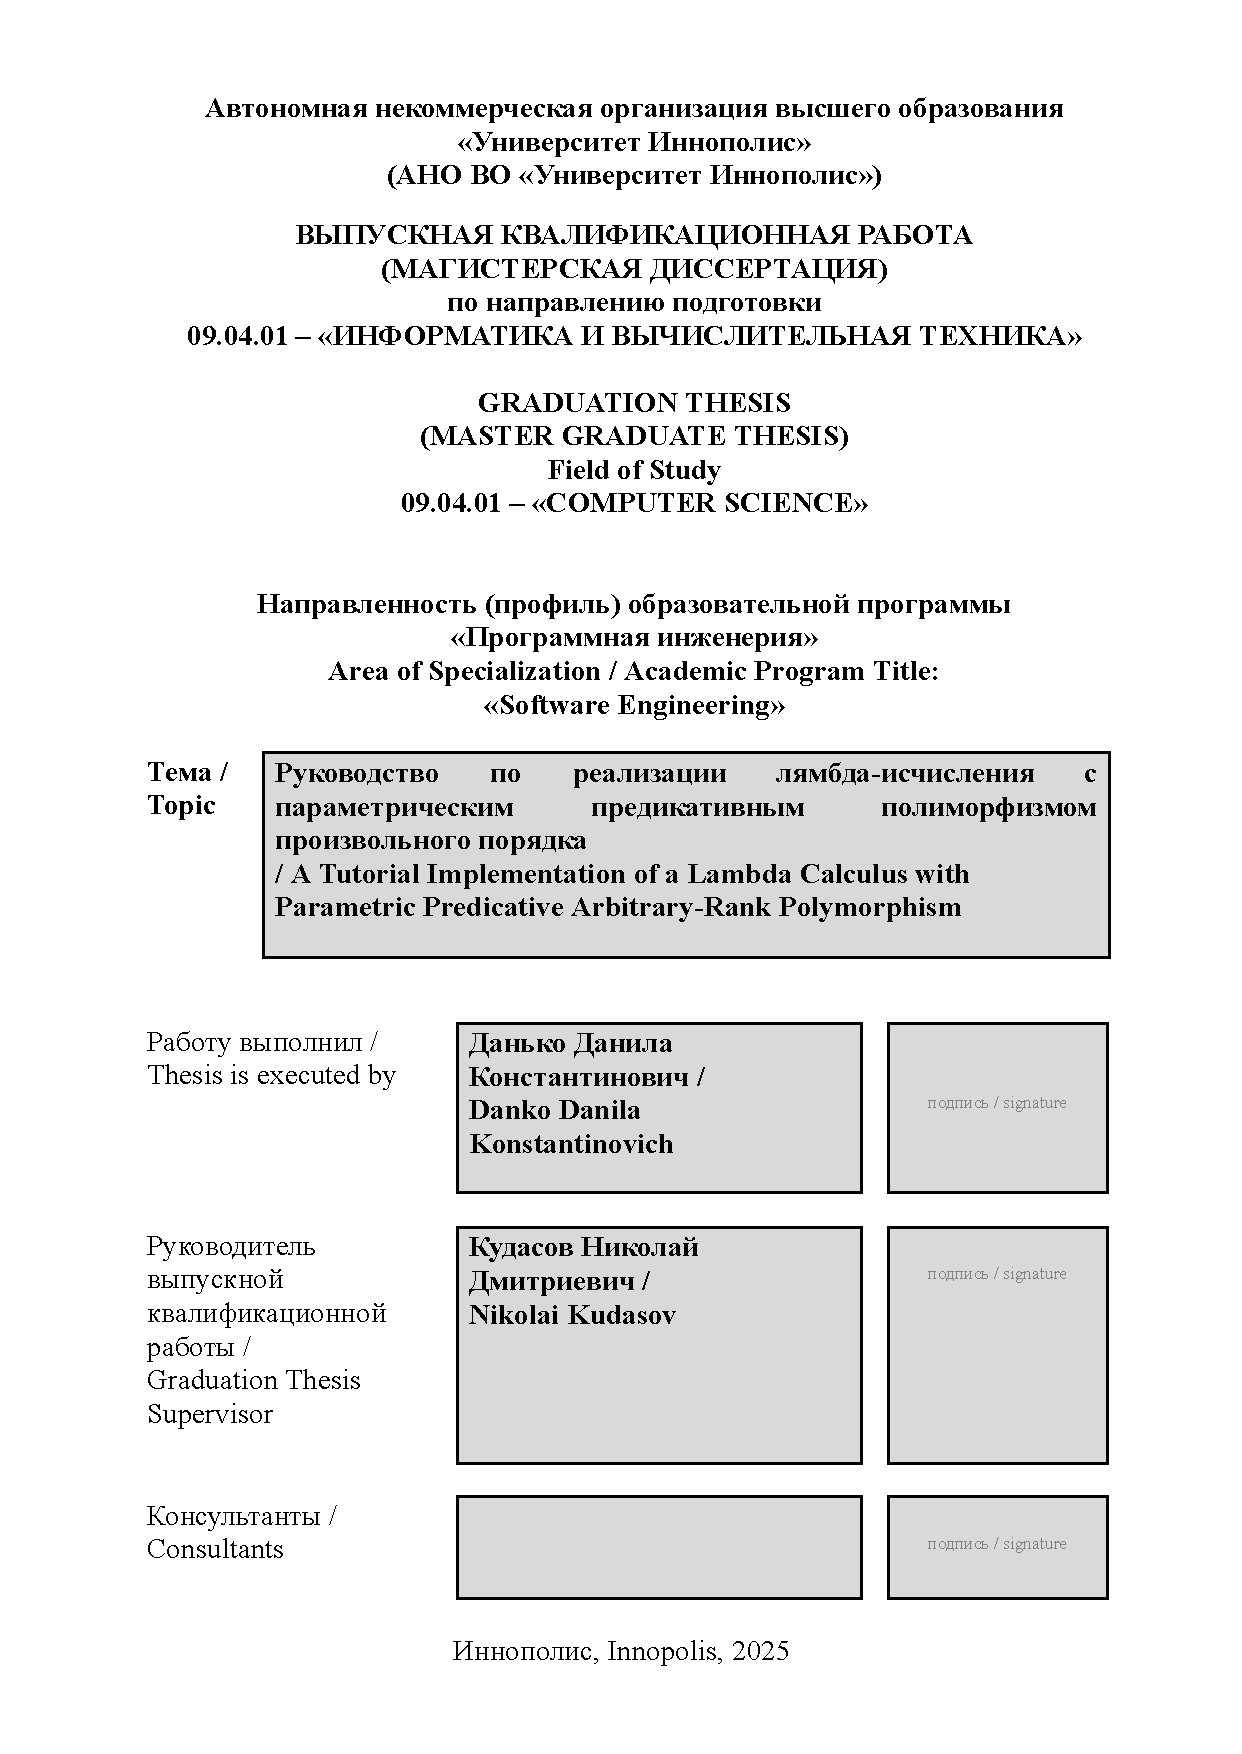
\includepdf[noautoscale,offset=75 -75,pages=-]{title.pdf}

% \setcounter{page}{2}

\tableofcontents

\cleardoublepage
\listoftables

\cleardoublepage
\listoffigures

\cleardoublepage
\begin{abstract}

\dots

\end{abstract}

% Depend on above part

\setcounter{page}{8}

% set manually the number, from which Chapter 1 starts!
% Why do we put 7 in this case?
% Title page - page 1
% Contents - page 2, page 3
% List of tables - page 4
% List of figures - page 5
% Abstract - page 6
% Chapter 1 - page 7
% In your thesis the counter number can be different, please count carefully and insert the corresponding number.

\chapter{Introduction}
\label{chap:Introduction}

\epigraph{Any sufficiently advanced technology is indistinguishable from magic.}{\textit{Arthur C. Clarke}}

For me, the Glasgow Haskell Compiler (GHC) \cite{ghc-site-2025} represented that "sufficiently advanced technology." Despite programming in Haskell for several years prior to beginning this thesis, I had not yet explored the internal workings of its primary compiler, which remained a source of profound curiosity.

As one of the most advanced and widely-used compilers for a functional programming language, the Glasgow Haskell Compiler (GHC) serves as a benchmark for research and development in type systems. However, a key challenge in understanding systems like GHC is the pedagogical gap between academic theory and production code. While GHC's design is documented in seminal papers like "Practical Type Inference for Arbitrary-Rank Polymorphism" \cite{jones-practical-2007}, these resources can be difficult for learners to approach. The academic literature is often theoretically dense, while GHC's source code is a large, highly-optimized production system, which can hide the core algorithms.

This thesis aims to bridge this gap. It presents the design and implementation of a small, typed functional language called Arralac (\textbf{Ar}bitrary-\textbf{ra}nk polymorphism + \textbf{la}mbda \textbf{c}alculus). This project serves as a tutorial implementation of arbitrary-rank polymorphism. By using modern architectural patterns from GHC - such as the "Trees that Grow" AST representation and level-based scoping for unification - in a focused and simplified context, this work provides a clear path for understanding these advanced concepts.

The central thesis of this work is that a focused, well-documented implementation can serve as a more accessible learning tool for advanced type systems than studying the original papers or production compilers directly. To support this, the project includes a complete toolchain, featuring a parser, interpreter, and a Language Server Protocol (LSP) implementation for an interactive development experience.

To guide this work, the following research questions are addressed:
\begin{enumerate}
    \item How can the core algorithms for type inference with arbitrary-rank polymorphism be implemented in a clear and step-by-step manner?
    \item How can compiler implementation patterns from GHC, like "Trees that Grow" and level-based unification, be simplified for an educational setting while retaining their key benefits?
    \item How can the Language Server Protocol be used to create an interactive development experience that helps in understanding a language's type system?
\end{enumerate}

The resulting implementation is publicly available on GitHub \cite{deemp-arbitrary-rank-tutorial} under the MIT license to serve as a resource for the community, aiming to fill the observed gap in well-documented, GHC-like educational compilers.

\section{Overview}

This thesis is structured as follows:

\Cref{chap:LiteratureReview} reviews existing approaches to building parts of the desired system.
Subsequently, \Cref{chap:DesignImplementation} explains my technical decisions and details the theoretical foundations.
\Cref{chap:EvaluationDiscussion} evaluates the results obtained and discusses the development process and experience.
Following this, \Cref{chap:Conclusion} outlines potential directions for future work.
% TODO does it?
% Finally, \Cref{chap:Appendix} contains relevant code snippets referenced throughout the thesis.

\chapter{Literature Review}
\label{chap:LiteratureReview}

\section{The Foundations of Typed Functional Languages}
\label{sec:LitReviewFoundations}

At the heart of modern, statically-typed functional languages like Haskell and OCaml lies a sophisticated type system \cite{haskell-type-systems-research, ocaml-papers}, a collection of formal rules assigning a property, or \textbf{type}, to every construct in a program \cite{pierce-types-2002}. A well-typed program is guaranteed to be free from a large class of runtime errors, such as applying an arithmetic operation to a string, a crucial property known as \textbf{type safety}. The theoretical basis for these languages is the \textbf{Lambda Calculus}, a formal system for expressing computation through function abstraction and application.

The most foundational typed variant is the \textbf{Simply-Typed Lambda Calculus (STLC)}. It ensures type safety by requiring every function parameter to be explicitly annotated with a type, and it verifies that functions are only ever applied to arguments of the matching type \cite{Pierce-SF2}. For example, the boolean \texttt{not} function, \texttt{\textbackslash(x : Bool). if x then false else true}, is correctly assigned the type \texttt{Bool -> Bool}.

However, STLC's safety comes at the cost of expressivity. The system is fundamentally \textbf{monomorphic}: each function can only have one, specific type. An identity function, for instance, can be written for booleans (\texttt{\textbackslash(x~:~Bool).~x}) or for integers (\texttt{\textbackslash(x~:~Int).~x}), but a single, universal identity function that works for \textit{all} types is impossible to express. This inherent rigidity makes pure STLC impractical for building reusable, large-scale software and creates a fundamental need for more expressive polymorphic systems.

\section{System F: The Ideal of Polymorphism and its Practical Limits}
\label{chap:LiteratureReview:sec:PolymorphismAndSystemF}

To overcome the limitations of monomorphism, modern languages rely on \textbf{polymorphism}, which allows a single piece of code to operate on values of multiple types. The foundational system that formally introduced this capability is Jean-Yves Girard's \textbf{System F} \cite{girard-system-f}. System F extends the lambda calculus with type abstraction and type application, enabling the creation of truly generic functions through what is known as \textbf{parametric polymorphism}. In System F, a universal identity function can be written with the polymorphic type \texttt{forall a. a -> a}, where the \texttt{forall} quantifier introduces a \textbf{type variable} \texttt{a} that can be instantiated with any concrete type at the function's call site.

Within such powerful systems, a crucial distinction exists between predicative and impredicative polymorphism. In a \textbf{predicative} system, a quantified type variable (like \texttt{a}) can only be instantiated with a \textbf{monotype} --- a simple type that does not itself contain any \texttt{forall} quantifiers. In contrast, a more powerful \textbf{impredicative} system allows a type variable to be instantiated with another \textbf{polytype}. While this "first-class" polymorphism is highly expressive, full type inference for impredicative systems is undecidable \cite{wells-typability-1999, serrano-quick-2020}. This fundamental trade-off between expressive power and decidability directly informs the scope of this thesis, which, following the pragmatic tradition of GHC \cite{jones-practical-2007}, operates within the simpler and more predictable predicative fragment.

\section{Practical Polymorphism: The Hindley-Milner Compromise and the Rank-N Gap}
\label{sec:LitReviewHM}

While System F provides the theoretical ideal for polymorphism, its power makes it impossible to create an algorithm that can always infer a program's types without explicit annotations from the programmer. To make type inference both practical and automatic, languages like ML adopted a decidable and well-behaved subset of System F known as the \textbf{Damas-Hindley-Milner (HM)} type system \cite{damas-milner}.

The practicality of the HM system stems from a foundational compromise: it only supports \textbf{Rank-1} types. This restriction means that \texttt{forall} quantifiers are only permitted at the very outermost level of a type definition. For example, \texttt{forall a. a -> Int} is a valid Rank-1 type, but a type where the quantifier is nested, such as \texttt{(forall a. a -> a) -> Int}, is known as a \textbf{higher-rank type} (specifically, a Rank-2 type) and is forbidden in a standard HM system.

This Rank-1 restriction is the key to the system's tractability, ensuring that type inference is decidable and can be implemented efficiently by algorithms like Algorithm W \cite{jones-practical-2007}. However, this compromise simultaneously introduces a significant expressive limitation: the "Rank-N gap". It becomes impossible to pass a polymorphic function as an argument to another function, as doing so would require a higher-rank type. This "Rank-N gap" represents the central challenge that must be overcome to support many powerful functional programming idioms, motivating the development of more sophisticated, yet still practical, type systems.

\section{A Practical Solution for Higher Ranks}
\label{sec:LitReviewJones2007}

The definitive solution to the Rank-N gap within a practical compiler context was presented in \textit{Practical type inference for arbitrary-rank types} by Peyton Jones et al. \cite{jones-practical-2007}. This seminal paper provides the direct theoretical and architectural foundation for this thesis. Rather than attempting full, undecidable inference, the authors propose a system that extends the predictable Hindley-Milner framework by cleverly leveraging programmer-supplied type annotations to guide the typechecker.

The core contribution is a \textbf{bidirectional type inference algorithm}. The system operates in two modes: an \textbf{inference mode} that synthesizes the most general type for an expression, and a \textbf{checking mode} that verifies an expression against a known, expected type. This duality is the key to its practicality: when a higher-rank type is required (e.g., as a function argument), programmer annotations are used to switch the algorithm into the more constrained checking mode, thereby avoiding the need for full inference while still enabling the use of polymorphic arguments.

To correctly handle the "more polymorphic than" relationship between types, the algorithm introduces a robust \textbf{subsumption} check. The mechanical heart of this check is a technique called \textbf{deep skolemization}, which correctly and efficiently handles quantifiers nested within function types. The detailed mechanics of this algorithm, including the type hierarchy ($\sigma, \rho, \tau$), the monotype invariant for unification, and the contravariant handling of function arguments, will be presented in \Cref{chap:DesignAndMethodology} as they form the direct basis for the implementation in this thesis.

\section{The Modern Landscape of Bidirectional Typing}
\label{chap:LiteratureReview:sec:TypeInferenceAlgorithm}

The bidirectional system from \cite{jones-practical-2007} provides the foundation for this thesis, but the field has continued to evolve. This section surveys key subsequent developments, contextualizing the chosen approach and further justifying its suitability for a pedagogical project. The continued interest in bidirectional typing is evidenced by numerous publicly available implementations, which serve as valuable resources for researchers and students alike \cite{github-goldenberg-artem-goldenbergbidirectionalsystem-2025, github-choi-kwanghoonbidi-2025, github-chen-cu1ch3ntype-inference-zoo-2025}.

\subsection{The Rise of Formal Bidirectional Systems}

A significant thread of modern research has focused on placing bidirectional typing on a more rigorous formal foundation. \citeauthor{dunfield-complete-2013} \cite{dunfield-complete-2013} presented a declarative, bidirectional algorithm for higher-rank predicative polymorphism, proving its soundness and completeness with respect to System F \cite{selinger-lecture-2013}. This foundational work, extended by \citeauthor{dunfield-sound-2019} in \cite{dunfield-sound-2019} and surveyed in \cite{dunfield-bidirectional-2020}, provides a clean type-theoretic basis using ordered contexts, in contrast to the more operational, constraint-based techniques of GHC.

\subsection{Refining and Generalizing Bidirectional Typing}

Subsequent research has focused on refining the bidirectional model. \citeauthor{xie-higher-rank} \cite{xie-higher-rank} proposed refinements to the algorithm from \cite{dunfield-complete-2013}, while more recently, \citeauthor{xue-contextual-2024} \cite{xue-contextual-2024} generalized the approach to \textbf{contextual typing}, allowing for more fine-grained propagation of type information.

\subsection{Exploring Alternatives: Impredicativity and Subtyping}

In parallel, another line of research has explored supporting full, first-class impredicativity. \citeauthor{parreaux-when-2024} \cite{parreaux-when-2024} propose \textbf{SuperF}, a novel algorithm that supports impredicativity by replacing unification with \textbf{subtype inference}\footnote{The SuperF implementation can be found at \url{https://github.com/hkust-taco/superf}.}. While extremely powerful, this approach represents a significant departure from the unification-based systems that are the focus of this thesis.

\subsection{Justification of the Chosen Approach}

This survey confirms that while many innovative approaches exist, the practical, predicative, and unification-based system pioneered in \cite{jones-practical-2007} remains the most suitable foundation for this project. The formal systems of Dunfield et al. are elegant but are further removed from the concrete implementation techniques (like constraint solving and mutable metavariables) used in GHC. The subtyping-based approach of SuperF is a different paradigm entirely.

Therefore, for the pedagogical goals of this thesis --- to create a tutorial implementation that demystifies a production-grade approach --- basing the work on the established and practical foundation of Jones et al. is the most direct and effective strategy. It provides a clear path to understanding the core challenges of higher-rank types and the architectural patterns used to solve them in a real-world compiler.

\chapter{Design and Methodology}
\label{chap:DesignAndMethodology}

This chapter details the architectural design and core methodologies employed in the implementation of \texttt{Arralac}, a tutorial compiler for a lambda calculus with arbitrary-rank polymorphism. The design is heavily inspired by the bidirectional type inference system described in \textit{Practical type inference for arbitrary-rank types} \cite{jones-practical-2007}, but it incorporates several modern implementation techniques and diverges in key areas to prioritize clarity and extensibility. This chapter will first outline the overall system architecture, then justify the choice of Abstract Syntax Tree (AST) representation, and finally, delve into the specifics of the constraint-based type inference engine and the methodology used to validate its correctness.

\section{System Architecture: The Compilation Pipeline}
\label{sec:Design:Pipeline}

The process of transforming a source file from plain text into an evaluated term is managed by a multi-stage pipeline, depicted in \Cref{fig:pipeline}. Each stage performs a distinct transformation on the program representation, passing its output to the next. This standard pipeline structure \cite{wits-type-inference-using-constraints} was chosen to promote modularity and a clear separation of concerns, which are essential for creating an understandable and maintainable tutorial compiler.

\begin{figure}[h!]
    \centering
    \begin{tikzpicture}[
            node distance=1.5cm and 2.5cm,
            auto,
            block/.style={rectangle, draw, fill=blue!20, text width=7em, text centered, rounded corners, minimum height=3em},
            arrow/.style={-Latex, thick}
        ]
        % Define the pipeline stages as nodes
        \node[block] (reader) {Reading};
        \node[block, right=of reader] (parser) {Parsing};
        \node[block, right=of parser] (renamer) {Renaming};
        \node[block, below=of renamer] (typechecker) {Typechecking};
        \node[block, left=of typechecker] (solver) {Solving};
        \node[block, left=of solver] (zonker) {Zonking};
        \node[block, below=of zonker] (core) {Core Conversion};
        \node[block, right=of core] (evaluation) {Evaluation};

        % Draw the arrows connecting the stages
        \draw[arrow] (reader) -> (parser);
        \draw[arrow] (parser) -> (renamer);
        \draw[arrow] (renamer) -> (typechecker);
        \draw[arrow] (typechecker) -> (solver);
        \draw[arrow] (solver) -> (zonker);
        \draw[arrow] (zonker) -> (core);
        \draw[arrow] (core) -> (evaluation);
    \end{tikzpicture}
    \caption{The \texttt{Arralac} Compilation Pipeline.}
    \label{fig:pipeline}
\end{figure}

The stages are as follows:
\begin{itemize}
    \item \textbf{Reading \& Parsing:} The source text is read and transformed by a BNFC-generated parser \cite{bnfc-site-2025} into an initial AST, with each node annotated with its source location.
    \item \textbf{Renaming:} This stage performs $\alpha$-conversion, assigning a unique identifier to every variable binding to resolve shadowing and prepare the program for typechecking.
    \item \textbf{Typechecking (Constraint Generation):} The renamed AST is traversed to generate a set of type constraints. This pass gathers equality and implication constraints but does not solve them.
    \item \textbf{Solving:} A separate iterative solver pass attempts to unify variables with types in the generated constraints, performing skolem escape and occurs checks.
    \item \textbf{Zonking:} After solving, a final pass substitutes all solved metavariables with their inferred types, producing a fully-typed AST.
    \item \textbf{Core Conversion:} The final, zonked AST is converted into a simpler Core language.
    \item \textbf{Evaluation:} The term in that Core language is evaluated to its weak head normal form (WHNF).
\end{itemize}

\section{Abstract Syntax Tree Design}
\label{sec:Design:AST}

The choice of AST representation is a foundational design decision. My design was guided by several key technical constraints: extensibility for future language features, the ability to annotate nodes for tooling, and smooth integration with the BNFC parser generator.

\subsection{Evaluating AST Representation Strategies}
Several alternatives were considered to meet these constraints. While the default AST generated by BNFC is simple and integrates perfectly with the parser, it lacks the necessary structural flexibility for a multi-pass compiler because it is too close to the concrete language syntax.

% TODO TTG uses type families
Libraries like \texttt{hypertypes} \cite{hypertypes-hackage} and \texttt{compdata} \cite{compdata-hackage} offer powerful approaches to building extensible ASTs, serving as a solution to the Expression Problem \cite{wadler-expression-1998}. However, they introduce a significant degree of a conceptual overhead that was deemed counterproductive for a tutorial project aimed at clarifying compiler internals.

Therefore, the \textbf{Trees That Grow (TTG)} pattern was selected \cite{trees-that-grow-2016}. It strikes an ideal balance, offering the extensibility needed for a phased compiler while remaining conceptually straightforward. It directly models the evolution of the AST through different stages, making it a powerful pedagogical tool in its own right and mirroring the architecture of GHC \cite{ghc-gitlab-2025}.


% TODO no extension field
My implementation of TTG differs slightly from GHC's. Whereas GHC uses concrete types in some fields, my implementation uses type family applications for \textit{all} fields, ensuring that every part of an AST node can be customized for a given compiler pass. Another difference is that I did not yet introduce an additional constructor for extending data types defined in the TTG representation because I did not expect usage of these types outside of the \texttt{Arralac} compiler.

\begin{figure}
    \centering
    \begin{minted}[frame=lines]{haskell}
    -- In GHC (compiler/Language/Haskell/Syntax/Expr.hs)
    data HsExpr p
      = HsVar (XVar p) (LIdP p) -- LIdP is a type synonym, not a type family
      ...
    
    type LIdP p = XRec p (IdP p)
    \end{minted}
    \caption{GHC's TTG AST Structure (Simplified)}
\end{figure}

\begin{figure}
    \centering
    \begin{minted}[frame=lines]{haskell}
    -- In Arralac (Language/Arralac/Syntax/TTG/SynTerm.hs)
    data SynTerm x
      = SynTerm'Var (XSynTerm'Var' x) (XSynTerm'Var x) -- All fields use type families
      ...
    
    -- Type families for each field, defined separately
    type family XSynTerm'Var' x
    type family XSynTerm'Var x
    \end{minted}
    \caption{Arralac's TTG AST Structure}
\end{figure}

This uniform use of type families provides a type-safe guarantee that pass-specific information, such as inferred types, is only available in the AST after that pass has successfully completed.

\section{Type Inference and Constraint Solving}
\label{sec:Design:TypeInference}

The design of the \texttt{Arralac} typechecker required a concrete implementation of several core concepts from the bidirectional system of \cite{jones-practical-2007}. This section outlines these foundational mechanisms that the methodology must realize and then describes the significant architectural divergence taken in \texttt{Arralac}.

\subsection{Foundations from \textit{Practical Type Inference}}
\label{sec:Design:Foundations}

The design of \texttt{Arralac}'s typechecker, while architecturally distinct, is a direct evolution of the bidirectional system presented in \textit{Practical type inference for arbitrary-rank types} \cite{jones-practical-2007}. To fully appreciate the design choices made in \texttt{Arralac}, it is essential to first understand the foundational mechanisms of this influential system, which elegantly balances expressive power with practical, decidable inference.

\subsubsection{Type Hierarchy and Context.}
At its core, the system stratifies types into a precise hierarchy to manage polymorphism. The type context, denoted by \textbf{$\Gamma$}, maps program variables to their types.
\begin{itemize}
    \item \textbf{Monotypes ($\tau$-types):} These are simple types with no polymorphism whatsoever, such as \texttt{Int} or \texttt{Bool -> Int}. They form the bedrock of the system.
    \item \textbf{Polytypes ($\sigma$-types):} These are types that begin with a \texttt{forall} quantifier, such as \texttt{forall a. a -> a}. They introduce polymorphism.
    \item \textbf{Rho-types ($\rho$-types):} These are an intermediate category, representing types that can appear on the right-hand side of a function arrow or under a \texttt{forall}. In the full higher-rank system, a $\rho$-type can be either a $\tau$-type or a function type $\sigma_1 \rightarrow \sigma_2$.
\end{itemize}
This stratification is crucial for controlling where and how polymorphism can appear and be inferred.

\subsubsection{Metavariables and the Monotype Invariant.}
During inference, the typechecker encounters expressions whose types are not yet known. It handles this by creating placeholder types called \textbf{metavariables} (e.g., $\alpha$, \texttt{$\beta$}). These are temporary, flexible variables that are gradually refined as the algorithm gathers more information. The process of solving for these metavariables is called \textbf{unification}.

A cornerstone of the system's practicality is the \textbf{monotype invariant}: a metavariable can only ever be unified with a monotype ($\tau$-type). This restriction is what guarantees that type inference is decidable and, crucially, \textbf{order-independent}. If a metavariable could be unified with a polytype, the result of inference could depend on the order in which expressions were traversed, leading to unpredictable and non-deterministic behavior. By enforcing this invariant, the algorithm ensures that the principal type it infers is unique and consistent.

\subsubsection{The Bidirectional Algorithm.}
The master strategy for handling higher-rank types is the \textbf{bidirectional type checking} algorithm. Instead of a single, monolithic inference function, the system operates in two distinct modes, preventing the need for full, undecidable inference:
\begin{itemize}
    \item \textbf{Inference Mode ($\uparrow$):} This mode synthesizes or "infers" the most general type for an expression from the bottom up. In the paper's implementation, this corresponds to functions like \texttt{inferRho} and \texttt{inferSigma}. It is used for expressions where the type is not already known.
    \item \textbf{Checking Mode ($\downarrow$):} This mode verifies or "checks" an expression against a known, expected type that is pushed down from the surrounding context. This is implemented by functions like \texttt{checkRho} and \texttt{checkSigma}.
\end{itemize}
This duality is key. For most of the program, the system can infer types. However, when it encounters a programmer-supplied annotation for a higher-rank type (e.g., on a function argument), it switches to the more constrained checking mode, using the annotation to guide the process and avoid intractable search.

\subsubsection{Subsumption: The "More Polymorphic Than" Check.}
A central challenge is determining if a function can be used where a more-specific polymorphic type is expected. This is handled by a \textbf{subsumption} check, which formalizes the notion of one type being "more polymorphic than" another. In the paper's implementation, this is the role of the \texttt{subsCheck} function. The mechanics of subsumption rely on two dual concepts: instantiation and skolemization.

% TODO clarify using, bound, checking against. What is the relation to programmer-given signatures?
\begin{itemize}
    \item \textbf{Instantiation:} When \textit{using} a polymorphic value (e.g., calling a function bound to a $\sigma$-type), its quantified type variables are replaced with fresh metavariables. This process, handled by \texttt{instantiate}, makes the type usable in a specific context.

    \item \textbf{Deep Skolemization:} The more complex case is checking against a polymorphic type \texttt{forall a. T}. To do this, the algorithm replaces the quantified variable \texttt{a} with a new, rigid constant called a \textbf{skolem}. A skolem constant is unique and cannot be unified with any other type. If a skolem constant "escapes" its scope (\textbf{skolem escape}) during subsequent unification (e.g., by being unified with a metavariable from an outer scope), a type error is raised.

          For arbitrary-rank types like \texttt{T1 -> (forall a. T2)}, the \texttt{forall} is nested. \textbf{Deep skolemization} is the paper's crucial innovation to handle this. It first transforms the type into a \textbf{weak prenex form} using an auxiliary function, $pr(\sigma)$, which pulls nested quantifiers from the return types of functions to the outermost level. For example,

          \begin{equation}
              \begin{split}
                  pr(\forall c. (\forall a. a \rightarrow c) \rightarrow (\forall b. b \rightarrow c)) & = \\
                  \quad \quad =\forall b c. \rightarrow (\forall a. a \rightarrow c) \rightarrow b \rightarrow c
              \end{split}
          \end{equation}

          This makes all quantifiers accessible for skolemization, enabling a consistent and robust subsumption check.
\end{itemize}

Finally, when checking function types for subsumption, such as \\ \texttt{($\sigma_1~\rightarrow~\sigma_2)~\leq~(\sigma_3~\rightarrow~\sigma_4$)}, the algorithm respects \textbf{contravariance}. The argument types are checked in the opposite direction ($\sigma_3 \leq \sigma_1$), while the result types are checked in the same direction ($\sigma_2 \leq \sigma_4$).

These mechanisms --- a strict type hierarchy, the monotype invariant, bidirectional checking, and subsumption check via deep skolemization --- work in concert to create a system that is powerful enough to support higher-rank types yet constrained enough to remain practical and decidable. This is the foundational system that \texttt{Arralac} reinterprets through a modern, constraint-based lens.

\subsection{Architectural Divergence: A Constraint-Based Model}
\label{sec:Design:ArralacApproach}

While the theoretical underpinnings are rooted in \cite{jones-practical-2007}, the implementation of the inference mechanism diverges significantly. Instead of the \textbf{eager unification} described in the paper, where constraints are solved as they are discovered, \texttt{Arralac} adopts a \textbf{constraint-based} approach inspired by GHC. This architectural choice was made to enhance modularity and to lay a more robust foundation for high-quality error diagnostics, reflecting modern compiler practice. \Cref{tab:arch-comparison} summarizes the key differences.

\begin{table}[h!]
    \centering
    \small
    \caption{Comparison of Type Inference Architectures}
    \label{tab:arch-comparison}
    \begin{tabular}{p{0.2\textwidth} p{0.35\textwidth} p{0.35\textwidth}}
        \toprule
        \textbf{Feature}            & \textbf{\cite{jones-practical-2007} (Eager Unification)}                             & \textbf{\texttt{Arralac} (Constraint-Based)}                                                                                                                              \\
        \midrule
        \textbf{Unification}        & Solves constraints immediately as they are generated.                                & Gathers all constraints first; solves them in a separate, dedicated pass.                                                                                                 \\
        \textbf{Modularity}         & Inference logic is tightly coupled with unification logic.                           & The Typechecker (generation) and Solver (unification) are fully decoupled modules.                                                                                        \\
        \textbf{Error Reporting}    & Errors are reported at the first point of unification failure, which can be obscure. & Already reports the location of a sub-term where a constraint originated. Has the potential for holistic error analysis by examining all conflicting constraints at once. \\
        \textbf{Let-Generalization} & Requires a global type context traversal at the point of the \texttt{let}-binding.   & Not implemented, but the architecture permits solving of scoped constraints during type checking.                                                                      \\
        \bottomrule
    \end{tabular}
\end{table}

\newpage
This separation is realized through two primary constraint types:
\begin{enumerate}
    \item \textbf{Canonical Equality Constraints (\texttt{EqCt}):} Represent a required equality between a metavariable and a type.
    \item \textbf{Implication Constraints (\texttt{Implication}):} Capture the scoping of polymorphism. An implication bundles a set of skolem variables created at the ambient level with \textbf{wanted} \cite{wits-type-inference-using-constraints} constraints generated from checking an expression after incrementing the ambient level.
\end{enumerate}

Furthermore, \texttt{Arralac} manages polymorphism scoping using \textbf{levels}, a technique also used in modern compilers \cite{practical-type-inference-with-levels-2025}. Every variable is assigned an integer \texttt{TcLevel} at creation. The solver then enforces the skolem escape check by a simple rule: a metavariable at level $n$ cannot be unified with a type containing any free variable (skolem or a metavariable) from a level $m > n$ \footnote{See \href{https://github.com/ghc/ghc/blob/ed38c09bd89307a7d3f219e1965a0d9743d0ca73/compiler/GHC/Tc/Utils/Unify.hs\#L2589}{Note [Unification preconditions]}}.

\section{Validation Methodology}
\label{sec:Implementation:Methodology}

% TODO generate test cases
To validate the correctness of the implementation and ensure it meets its pedagogical goals, a methodology of targeted, feature-driven testing was employed. Rather than relying on a large, undifferentiated test suite, specific test cases were developed to exercise the core mechanisms of the arbitrary-rank type system and its implementation.

\begin{enumerate}
    \item \textbf{Correct Handling of Higher-Rank Polymorphism:} The primary validation case involved a program that requires passing a polymorphic function as an argument, similar to \texttt{Program1.arralac} (\cref{sec:Implementation:Results}). The successful typechecking and evaluation of this program served as the baseline validation that the core bidirectional algorithm, including subsumption and deep skolemization, was implemented correctly.

          % TODO compose this test
    \item \textbf{Skolem Escape and Level Checking:} A specific negative test case was created to ensure that a skolem variable could not escape its scope during unification. The test involved attempting to unify a metavariable with a type containing a skolem from a deeper scope. The expected outcome was a type error from the solver, which validated that the level-based checking mechanism was correctly preventing unsound unifications.

    \item \textbf{Language Server Functionality:} The interactive tooling was validated manually within Visual Studio Code. This involved checking that (a) hovering over identifiers displayed the correct, fully-zonked types as inferred by the pipeline, and (b) introducing syntactic or semantic errors (e.g., unbound variables) triggered appropriate and timely error diagnostics from the language server.
\end{enumerate}

While this methodology does not constitute a formal proof of correctness, it provides enough evidence that the key features of the system are implemented correctly and robustly, satisfying the primary objectives of the thesis.

\section{Summary of Design Choices and Limitations}
\label{sec:Design:Summary}

The design of \texttt{Arralac} makes several deliberate trade-offs to prioritize its tutorial nature and extensibility over feature completeness. The key design choices were:
\begin{itemize}
    \item An extensible \textbf{Trees That Grow} AST to support future language features and tooling annotations.
    \item A GHC-style, two-phase \textbf{constraint-based type inference} engine, which separates constraint generation from solving.
    \item \textbf{Level-based scoping} for skolem variables, providing an efficient mechanism for escape checking.
\end{itemize}

This design, however, comes with several limitations compared to a production compiler. The accompanying Technical Appendix to the paper \cite{practical-type-inference-proofs} provides proofs of soundness and completeness for the theoretical system, but this implementation does not attempt to formally prove its own correctness. The most notable limitations are:
\begin{itemize}
    \item \textbf{No \texttt{let}-generalization:} Local \texttt{let}-bindings are not generalized, a simplification suggested in \cite{vytiniotis-outsideinx-2011}.
    \item \textbf{No recursive \texttt{let}-bindings.} just like in \cite{jones-practical-2007}.
    \item \textbf{No floating-out of constraints:} The solver does not attempt to move equality constraints out of implications to enable further solving.
    \item \textbf{Untyped Core Language:} Unlike GHC and \cite{jones-practical-2007}, \texttt{Arralac} translates \texttt{SynTerm}s to a simple, untyped Core language, forgoing the powerful consistency checks that a typed intermediate language provides. This simplification was a deliberate trade-off to keep the focus of the thesis squarely on the front-end type inference algorithm.
    \item \textbf{Simplified Constraint Solving:} The solver does not rewrite Wanteds with Wanteds \footnote{See \href{https://github.com/ghc/ghc/blob/ed38c09bd89307a7d3f219e1965a0d9743d0ca73/compiler/GHC/Tc/Types/Constraint.hs\#L2415}{Note [Wanteds rewrite Wanteds]}} and only reports the first constraint that it could not solve, not all residual constraints.
\end{itemize}

\chapter{Implementation and Results}
\label{chap:ImplementationAndResults}

The previous chapter detailed the architectural design and core methodologies for the \texttt{Arralac} compiler. This chapter transitions from design to practice, describing the concrete Haskell implementation that realizes this architecture.

First, I will examine the implementation of the core data structures, particularly the Trees That Grow (TTG) Abstract Syntax Tree (AST). Next, I will detail the implementation of the type inference pipeline, focusing on the separation between constraint generation and solving. Finally, I will present concrete results, including the output of the typechecker and evaluator for a sample program and a demonstration of the functional Language Server Protocol (LSP) features.

\section{AST Implementation with Trees That Grow}
\label{sec:Implementation:AST}

As outlined in the design (\cref{sec:Design:AST}), the AST is built using the Trees That Grow (TTG) pattern to ensure extensibility and to facilitate annotations. The core data types, \texttt{SynTerm} for expressions and \texttt{SynType} for syntactic types, are parameterized by a type variable \texttt{x} that represents the current compiler pass (e.g., \texttt{CompRn} for Renamed, \texttt{CompTc} for Typechecked).

Unlike a simpler AST where fields have concrete types, every component of an \texttt{Arralac} AST node is defined by a type family. This allows the structure of a node to be radically different across passes. For example, the definition for \texttt{SynTerm} in the module \texttt{Language.Arralac.Syntax.TTG.SynTerm} is shown below.

\begin{minted}[frame=lines,label={The Generic \texttt{SynTerm} Data Type}]{haskell}
data SynTerm x
  = -- | \ (x :: a) -> x
    SynTerm'ALam (XSynTerm'ALam' x) (XSynTerm'ALam'Var x) 
                 (XSynTerm'ALam'Type x) (XSynTerm'ALam'Body x)
  | -- | (f x) :: Int
    SynTerm'Ann (XSynTerm'Ann' x) (XSynTerm'Ann'Term x) 
                (XSynTerm'Ann'Type x)
  -- ... other constructors
\end{minted}

These type families are then instantiated for each specific compiler pass. For the typechecking pass (\texttt{CompTc}), the extension point fields (e.g., \texttt{XSynTerm'Ann'}) are instantiated with a \texttt{TcAnno} record, which crucially contains the inferred type for that node. This demonstrates how the tree "grows" to hold new information.

\begin{minted}[frame=lines,label={Type Family Instantiation for the \texttt{Typechecked} Pass}]{haskell}
-- In Language.Arralac.Syntax.Local.SynTerm.Tc
type instance XSynTerm'Ann'Term CompTc = SynTerm CompTc
type instance XSynTerm'Ann'Type CompTc = SynType CompTc

-- In Language.Arralac.Syntax.Local.Extension.Tc
type instance XSynTerm'Ann' CompTc = TcAnno
data TcAnno = TcAnno { annoSrcLoc :: SrcSpan, annoType :: Expected TcType }
\end{minted}

This approach provides a type-safe way to ensure that pass-specific information, such as inferred types, is only available in the AST after that pass has successfully completed.

\section{The Type Inference and Solving Pipeline}
\label{sec:Implementation:Pipeline}

The implementation of the type inference engine closely follows the constraint-based design laid out in \cref{sec:Design:TypeInference}. The process is divided into distinct, sequential stages, each managed by its own set of modules.

\subsection{Constraint Generation (\texttt{Typechecker})}
The first phase, implemented primarily in the \\ \texttt{Language.Arralac.Typechecker.TcTerm} module, traverses the renamed AST to produce a set of wanted constraints. It does not perform any unification itself.
\begin{itemize}
  \item \textbf{Bidirectional Logic:} The core function, \texttt{tcRho}, implements the bidirectional algorithm. When called in inference mode (via the \texttt{inferRho} wrapper), it creates a new IORef to hold the resulting type. When called in checking mode (via \texttt{checkRho}), it consumes the expected type passed to it.

  \item \textbf{Implication Constraints:} At each point where skolemization is required---specifically, within the \texttt{checkSigma} function when checking an expression against a polymorphic type---the typechecker enters a deeper scope. This is implemented by the \texttt{pushLevelAndCaptureConstraints} helper function, which increments the current \texttt{TcLevel}, captures all new constraints generated within its scope, and packages them into an \texttt{Implic} constraint.
\end{itemize}

\subsection{Constraint Solving (\texttt{Solver})}
The set of \texttt{WantedConstraints} generated by the typechecker is passed to the solver, implemented in \texttt{Language.Arralac.Solver.Solve}. The solver iteratively processes the worklist of simple equality constraints (\texttt{wc\_simple}).
\begin{itemize}
  \item \textbf{Occurs and Level Checks:} Before attempting to unify a metavariable with a type, the solver performs two critical checks, implemented in \texttt{Language.Arralac.Solver.Check}. First, an \textbf{occurs check} ensures the metavariable does not appear within the right-hand side of the type, preventing infinite types. Second, a \textbf{level check} verifies that the type does not contain any skolem variables with a level deeper than the metavariable, thus enforcing the skolem escape rule.
  \item \textbf{Unification:} If the checks pass, the solver unifies the variable by writing to the metavariable's mutable reference (\texttt{IORef}). Constraints within implications are solved recursively within their own scope. Any constraints that cannot be solved (e.g., due to a type mismatch or a failed check) are currently dropped, and their metavariables remain unsolved.
\end{itemize}

\subsection{Finalization (\texttt{Zonker})}
After the solver has completed, the \texttt{Zonker}, implemented in \texttt{Language.Arralac.Zonker.Zn.Zonk}, traverses the now-typed AST. It recursively resolves the \texttt{IORef} of each metavariable, replacing it with its final, unified type. Metavariables that were not solved are explicitly renamed to indicate their status (e.g., \texttt{a_Unsolved_11}), producing a final AST that is free of mutable references and ready for code generation or evaluation.

\section{Results and System Characteristics}
\label{sec:Implementation:Results}

This section demonstrates the functionality of the implemented system using a concrete example and evaluates its characteristics based on the criteria from the thesis guidelines.

\subsection{A Complete Example}
To test the core functionality, I use a program that requires arbitrary-rank polymorphism: passing a polymorphic function as an argument. The following program, \texttt{Program1.arralac}, defines a function \texttt{applyMyShow} that expects a polymorphic function of type \texttt{forall b. b -> String} and applies it to a value.

\begin{minted}[frame=lines,label={Program1.arralac}]{haskell}
let
  applyMyShow =
    (\x. \y. x y)
      :: forall a. (forall b. b -> String) -> a -> String
in
let
  myShow = \x. "Hello"
in
applyMyShow myShow
\end{minted}

\subsection{Type Checking and Evaluation}
Running the \texttt{Arralac} CLI to typecheck the program produces a fully-annotated and pretty-printed AST. The output below shows that the system correctly inferred and propagated the types, including the higher-rank type of the lambda-bound variable \texttt{x\_1}.

\begin{figure}[h]
  \centering
  \begin{minted}[frame=lines]{console}
$ nix run .#arralac -- typecheck arralac/test/data/Program1.arralac

(let
  applyMyShow_0 = 
    (\(x_1 :: forall b_4. b_4 -> String).
       (\(y_2 :: a_9). (x_1 :: a_9 -> String) (y_2 :: a_9) :: String
       ) :: a_9 -> String
    ) :: (forall b_4. b_4 -> String) -> a_9 -> String
in
  (let myShow_7 = (\(x_8 :: b_13). "Hello") :: b_13 -> String
   in (applyMyShow_0 (myShow_7)) :: a_Unsolved_11 -> String
  ) :: a_Unsolved_11 -> String
) :: a_Unsolved_11 -> String
\end{minted}
  \caption{Typechecking output for \texttt{Program1.arralac}.}
  \label{fig:typecheck-output}
\end{figure}

Note the final type includes \texttt{a\_Unsolved\_11}, correctly indicating that the type variable \texttt{a} from the original signature was not constrained and thus remains unsolved.

The evaluator correctly reduces the program to its weak head normal form (WHNF):

\begin{figure}
  \centering
  \begin{minted}[frame=lines]{console}
$ nix run .#arralac -- evaluate whnf arralac/test/data/Program1.arralac

\y_2. (\x_8. "Hello") (y_2)
\end{minted}
  \caption{Evaluation output for \texttt{Program1.arralac}.}
  \label{fig:evaluate-output}
\end{figure}

\subsection{Language Server Functionality}
The implementation includes a functional language server that provides on-the-fly diagnostics and type information. \Cref{fig:lsp-demo} demonstrates two key features in Visual Studio Code: (1) hovering over an identifier (\texttt{applyMyShow}) to see its inferred polymorphic type, and (2) an error diagnostic for an unbound variable (\texttt{myShowww}).

\begin{figure}[h!]
  \centering
  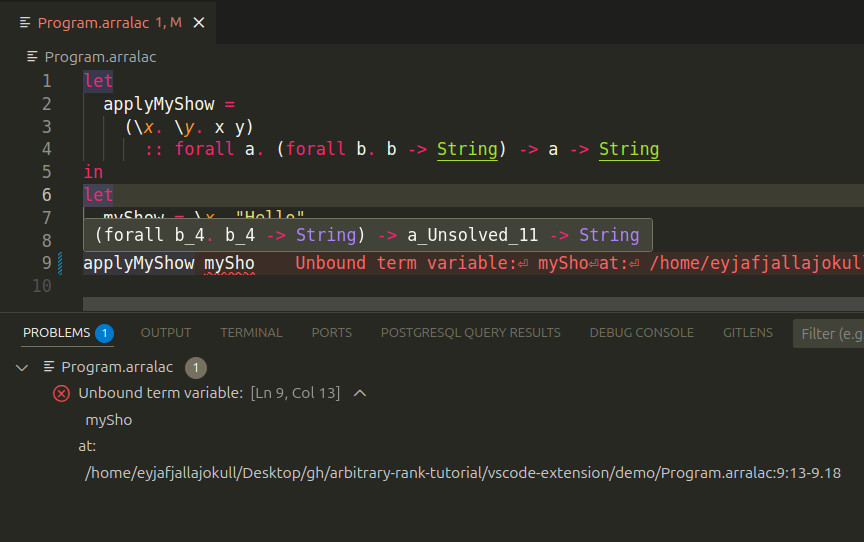
\includegraphics[width=0.9\textwidth]{VSCode.png}
  \caption{LSP features: type on hover and error diagnostics.}
  \label{fig:lsp-demo}
\end{figure}

\subsection{Codebase Characteristics}
The system was evaluated against several quality characteristics from ISO 25010.
\begin{itemize}
  \item \textbf{Modularity:} The codebase is highly modular, comprising 86 distinct Haskell modules, as shown by the \texttt{cloc} \footnote{The tool is available at \url{https://github.com/AlDanial/cloc}} analysis in \cref{table:cloc}. This separation of concerns was critical for managing the complexity of the type inference engine.
  \item \textbf{Analysability:} The error-handling mechanism is designed for clear diagnostics. Each pipeline stage (e.g., Renamer, Typechecker, Solver) throws its own distinct error type, which captures a full call stack. This ensures that failures are easy to trace back to their source.
  \item \textbf{Installability:} The entire project is packaged with Nix, enabling a reproducible, single-line installation via the command \texttt{nix profile install}.
\end{itemize}

\begin{table}[h!]
  \centering
  \footnotesize
  \caption{Code Metrics for the \texttt{Arralac} Implementation \\
    Generated by \texttt{cloc}}
  \begin{tabular}{lrrrr}
    \toprule
    \textbf{Language} & \textbf{Files} & \textbf{Blank Lines} & \textbf{Comment Lines} & \textbf{Code Lines} \\
    \midrule
    Haskell           & 86             & 705                  & 1085                   & 3907                \\
    \midrule
    \textbf{SUM}      & \textbf{86}    & \textbf{705}         & \textbf{1085}          & \textbf{3907}       \\
    \bottomrule
  \end{tabular}
\label{table:cloc}
\end{table}

This chapter has demonstrated that the design laid out previously has been successfully realized in a functional, well-structured, and non-trivial implementation. The system correctly handles higher-rank types and provides modern tooling, fulfilling the primary objectives of this thesis.

\chapter{Analysis and Discussion}
\label{chap:AnalysisAndDiscussion}

This chapter moves beyond description to provide a critical analysis of the \Arralac project. The analysis will proceed in three parts. First, I will evaluate how the chosen design patterns successfully achieved the project's primary objectives and what trade-offs they entailed. Second, I will offer a qualitative evaluation of the system's non-functional characteristics. Finally, I will critically examine the limitations of the current implementation and propose concrete directions for future research.

\section{Analyzing the Architectural Contributions}
\label{sec:Discussion:Objectives}

The primary goal of this thesis was to create a modern, tutorial-focused implementation of arbitrary-rank polymorphism by synthesizing foundational theory with modern compiler engineering practices.

\subsection[From Eager Unification to Constraint-Based Inference]{From Eager Unification \\ to Constraint-Based Inference}
The most significant architectural contribution of this work is its adoption of a two-phase, constraint-based type inference model, a departure from the eager unification algorithm presented in \cite{jones-practical-2007}. In their paper, the authors suggest that a "more principled alternative is to... get the inference algorithm to return a set of constraints, and solve them all together" \cite[Sec. 9.6]{jones-practical-2007}.

\Arralac serves as a direct, working implementation of this suggestion. By separating constraint generation (the \texttt{Typechecker}) from constraint solving (the \texttt{Solver}), this thesis demonstrates that the benefits of this architecture are fundamental to building a modular and understandable system.

\paragraph{Architectural Benefits and Trade-offs}
This separation yielded two primary benefits:
\begin{enumerate}
    \item \textbf{Improved Modularity:} The logic of the typechecker and solver are cleanly decoupled. The \texttt{Typechecker}'s sole responsibility is to traverse the AST and emit a declarative set of \texttt{WantedConstraints}. The \texttt{Solver} operates on this abstract set of constraints, free from the complexities of AST traversal.
    \item \textbf{A Foundation for Better Error Reporting:} A constraint-based model enables a holistic view of type errors. By gathering all constraints before solving, a future version of the solver could analyze the full set of conflicts to produce a much richer diagnostic than an eager unifier that fails on the first error.
\end{enumerate}

The primary trade-off is the added complexity of the \texttt{WantedConstraints} data structure, which becomes the sole interface between the two largest components of the inference engine. This required careful engineering to ensure all necessary context, such as source locations and levels for scope checking, was correctly propagated.

\subsection{The Trees That Grow AST: A Necessity for Modern Tooling}
The second key architectural choice was the adoption of the \textbf{Trees That Grow} (TTG) pattern for the AST. The LSP requires annotating the AST with inferred types, and TTG provides a type-safe and elegant solution. As demonstrated in \Cref{sec:Implementation:AST}, the AST is parameterized by the compiler pass, and type families are used to "grow" the tree with annotations like \texttt{TcAnno} only after the typechecking pass. This provides a compile-time guarantee that type information is not accessed before it has been computed.

\section[A Qualitative Evaluation of System Characteristics]{A Qualitative Evaluation \\ of System Characteristics}
\label{sec:Discussion:Characteristics}
Evaluating \Arralac against ISO 25010 \cite{iso-25010} sub-characteristics reveals the practical impact of its design.

\begin{itemize}
    \item \textbf{Modularity:} The division of the codebase into 86 modules (\Cref{table:cloc}) is a direct outcome of the pipeline architecture. The strict separation between stages creates a highly modular system. This modularity makes the codebase highly \textbf{analysable}; a student can study the \texttt{Solver} in isolation.
    \item \textbf{Analysability (Error Handling):} The system's analysability is enhanced by its error handling strategy. By defining distinct error types for each pipeline stage, each capturing a full call stack, the system provides transparent diagnostics.
    \item \textbf{Installability and Portability:} The use of Nix for dependency management and installation is critical to the project's goal of being a reproducible tutorial artifact. It guarantees that any (Linux or macOS) user can build and run the software with a single command.
\end{itemize}

\section{Limitations and Avenues for Future Work}
\label{sec:Discussion:Limitations}
A critical analysis requires acknowledging the project's limitations. These simplifications, however, suggest clear directions for future research.

\begin{enumerate}
    \item \textbf{Lack of \texttt{let}-generalization:} The most significant functional limitation is the lack of ML-style generalization for local \texttt{let}-bindings. Future work could add a scoped-solving phase at each \texttt{let}-binding, quantifying over any metavariables whose level is local to the binding's scope, as discussed in \cite{wits-type-inference-using-constraints}.

    \item \textbf{Untyped Core Language:} \Arralac desugars its typed AST into an untyped lambda calculus. A major extension would be to design a typed Core language and extend the desugaring process to generate the necessary type abstractions and applications, making the entire pipeline type-safe.

    \item \textbf{Simplified Constraint Solver:} The current solver is basic. It halts on the first unsolvable constraint and does not implement advanced strategies, like floating constraints out of implications and promotion \footnote{See \href{https://github.com/ghc/ghc/blob/ed38c09bd89307a7d3f219e1965a0d9743d0ca73/compiler/GHC/Tc/Utils/Unify.hs\#L2589}{Note [Unification preconditions]}}. Enhancing the solver to handle these cases and to report a complete set of residual constraints would be a valuable research project.
\end{enumerate}

In conclusion, the analysis confirms that \Arralac is not merely a \\ reimplementation, but a modernization of the ideas in its foundational literature. It successfully serves its pedagogical purpose while providing a robust foundation for future exploration.

\chapter{Conclusion}
\label{chap:Conclusion}

This thesis was motivated by a significant pedagogical gap between the foundational theory of advanced type systems and the complex reality of their production-grade implementations. I began with the central claim that this gap could be bridged not by yet another theoretical paper, but by a modern, tutorial-focused compiler that makes the core engineering principles of a system like GHC tangible and interactive. The design and implementation of \Arralac, a lambda calculus with arbitrary-rank polymorphism, has served to validate this thesis.

To achieve this, \Arralac was built upon a synthesis of carefully chosen architectural patterns. By integrating a modular, constraint-based type inference pipeline with an extensible Trees That Grow AST, the project established a foundation that is both robust and clear. This architecture was then brought to life through a complete toolchain, most notably a functional Language Server Protocol (LSP) implementation, which transforms the abstract algorithms of type inference into an explorable, interactive experience.

The development of \Arralac yielded a key insight: the architectural choices made in a compiler's design have a profound and direct impact on its pedagogical value. The separation of constraint generation from solving does not merely improve modularity; it creates an explicit representation of the typechecker's "reasoning" that can be inspected and understood in an easier way that an eager algorithm. Similarly, the use of the LSP confirms that modern tooling is a transformative element in computer science education. Providing on-the-fly type information and diagnostics directly within an editor makes the behavior of the type system immediately visible, turning abstract rules into concrete feedback.

While \Arralac successfully demonstrates its core thesis, its journey as a practical tool is far from complete. The logical next step is to tackle the crucial feature of \texttt{let}-generalization, a challenge for which the existing constraint-based architecture is an ideal foundation. Subsequently, evolving the evaluator to use a typed Core language would introduce the end-to-end type safety characteristic of production compilers. Extending the language server to support richer features, such as "go to definition," would further enhance its utility as a development and learning environment.


\enlargethispage{\baselineskip}
This thesis began with the goal of demystifying the "magic" of a production-grade type system. Through the design and implementation of \Arralac, it has shown that the core principles of arbitrary-rank polymorphism can be implemented in a structured, modern, and understandable way. By combining foundational theory with practical architectural patterns, this work provides a clear and interactive bridge for students, researchers, and aspiring language developers. Ultimately, this project stands as a testament to the idea that even the most powerful compiler technologies can be made accessible, fostering a deeper understanding and appreciation for the art of programming language implementation.


%% REFERENCES
\printbibliography[heading=bibintoc,title={Bibliography cited}]


% \appendix
\label{chap:Appendix}

\chapter{Extra Stuff}
\blindtext

\chapter{Even More Extra Stuff}
\blindtext

\end{document}

